%-*- coding: utf-8 -*-
\subsection{JavaScriptファイルの短縮化について}
\JS ファイルの短縮化を行う方法はいくつかあるが、ここでは、Google が提供
する Closure Compiler を紹介する
\footnote{\texttt{https://developers.google.com/closure/compiler/}
2016年11月23日参照}。

このサービスは次のように説明されている。
\begin{quotation}
The Closure Compiler is a tool for making JavaScript download and run
 faster. Instead of compiling from a source language to machine code, it
 compiles from JavaScript to better JavaScript. It parses your
 JavaScript, analyzes it, removes dead code and rewrites and minimizes
 what's left. It also checks syntax, variable references, and types, and
 warns about common JavaScript pitfalls.
 \end{quotation}
これによると、元来の\JS のコードをより良い\JS のコードに変換し、簡単な警
告を表示するようである。

使い方については次のように書かれている。
\begin{quotation}
 You can use the Closure Compiler as:

\begin{itemize}
 \item An open source Java application that you can run from the command
			 line.
 \item A simple web application.
 \item A RESTful API.
\end{itemize}
To get started with the compiler, see "How do I start" below.
\end{quotation}
ここでは2番目にある Web アプリケーションで行う。

このサイトは\texttt{http://closure-compiler.appspot.com/home}である(図
\ref{closure-compiler})。
 \begin{figure}[ht]
	\begin{center}
	 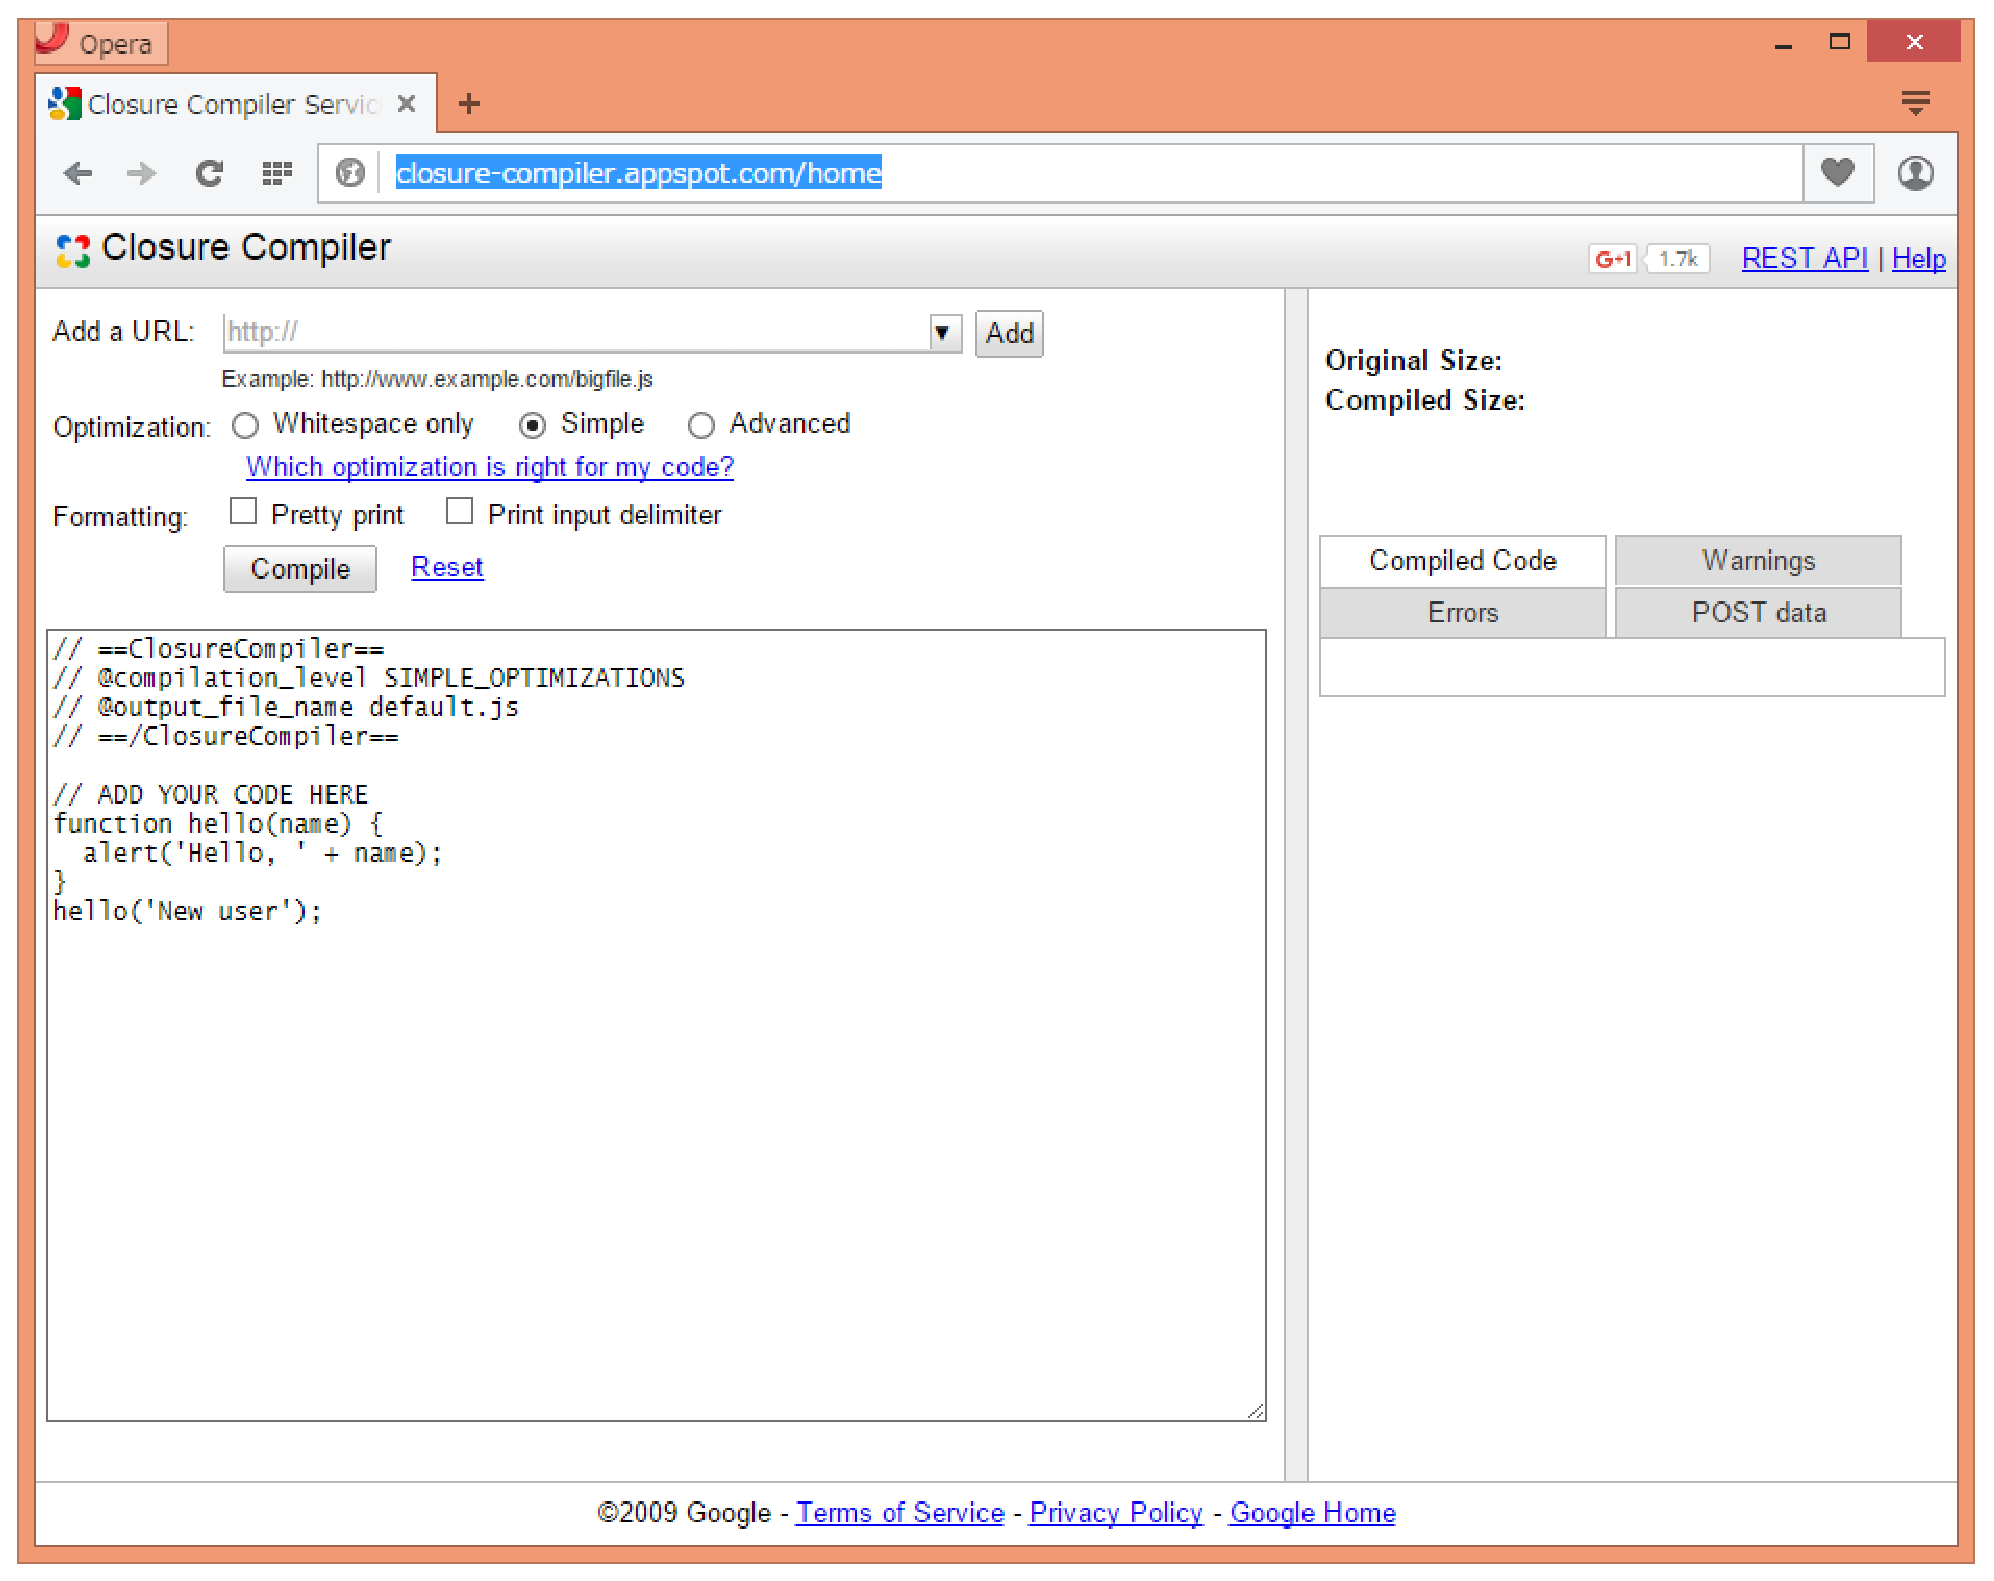
\includegraphics[width=0.9\textwidth]{10-01closur-compiler-home.eps}
	\end{center}
 \caption{Closure Compiler のホームページ}\label{closure-compiler}
 \end{figure}
 左側のテキストボックスにコードを張り付けて、「Compile」のボタンを押せば
 よい。
 %\newpage
\subsection{短縮化の例}
ここでは実行例\ref{EventInput}にある\texttt{event.js}で短縮化の効果を見
ることにする。

図\ref{closure-compiler-res02}はその結果である。
 \begin{figure}[ht]
	\begin{center}
	 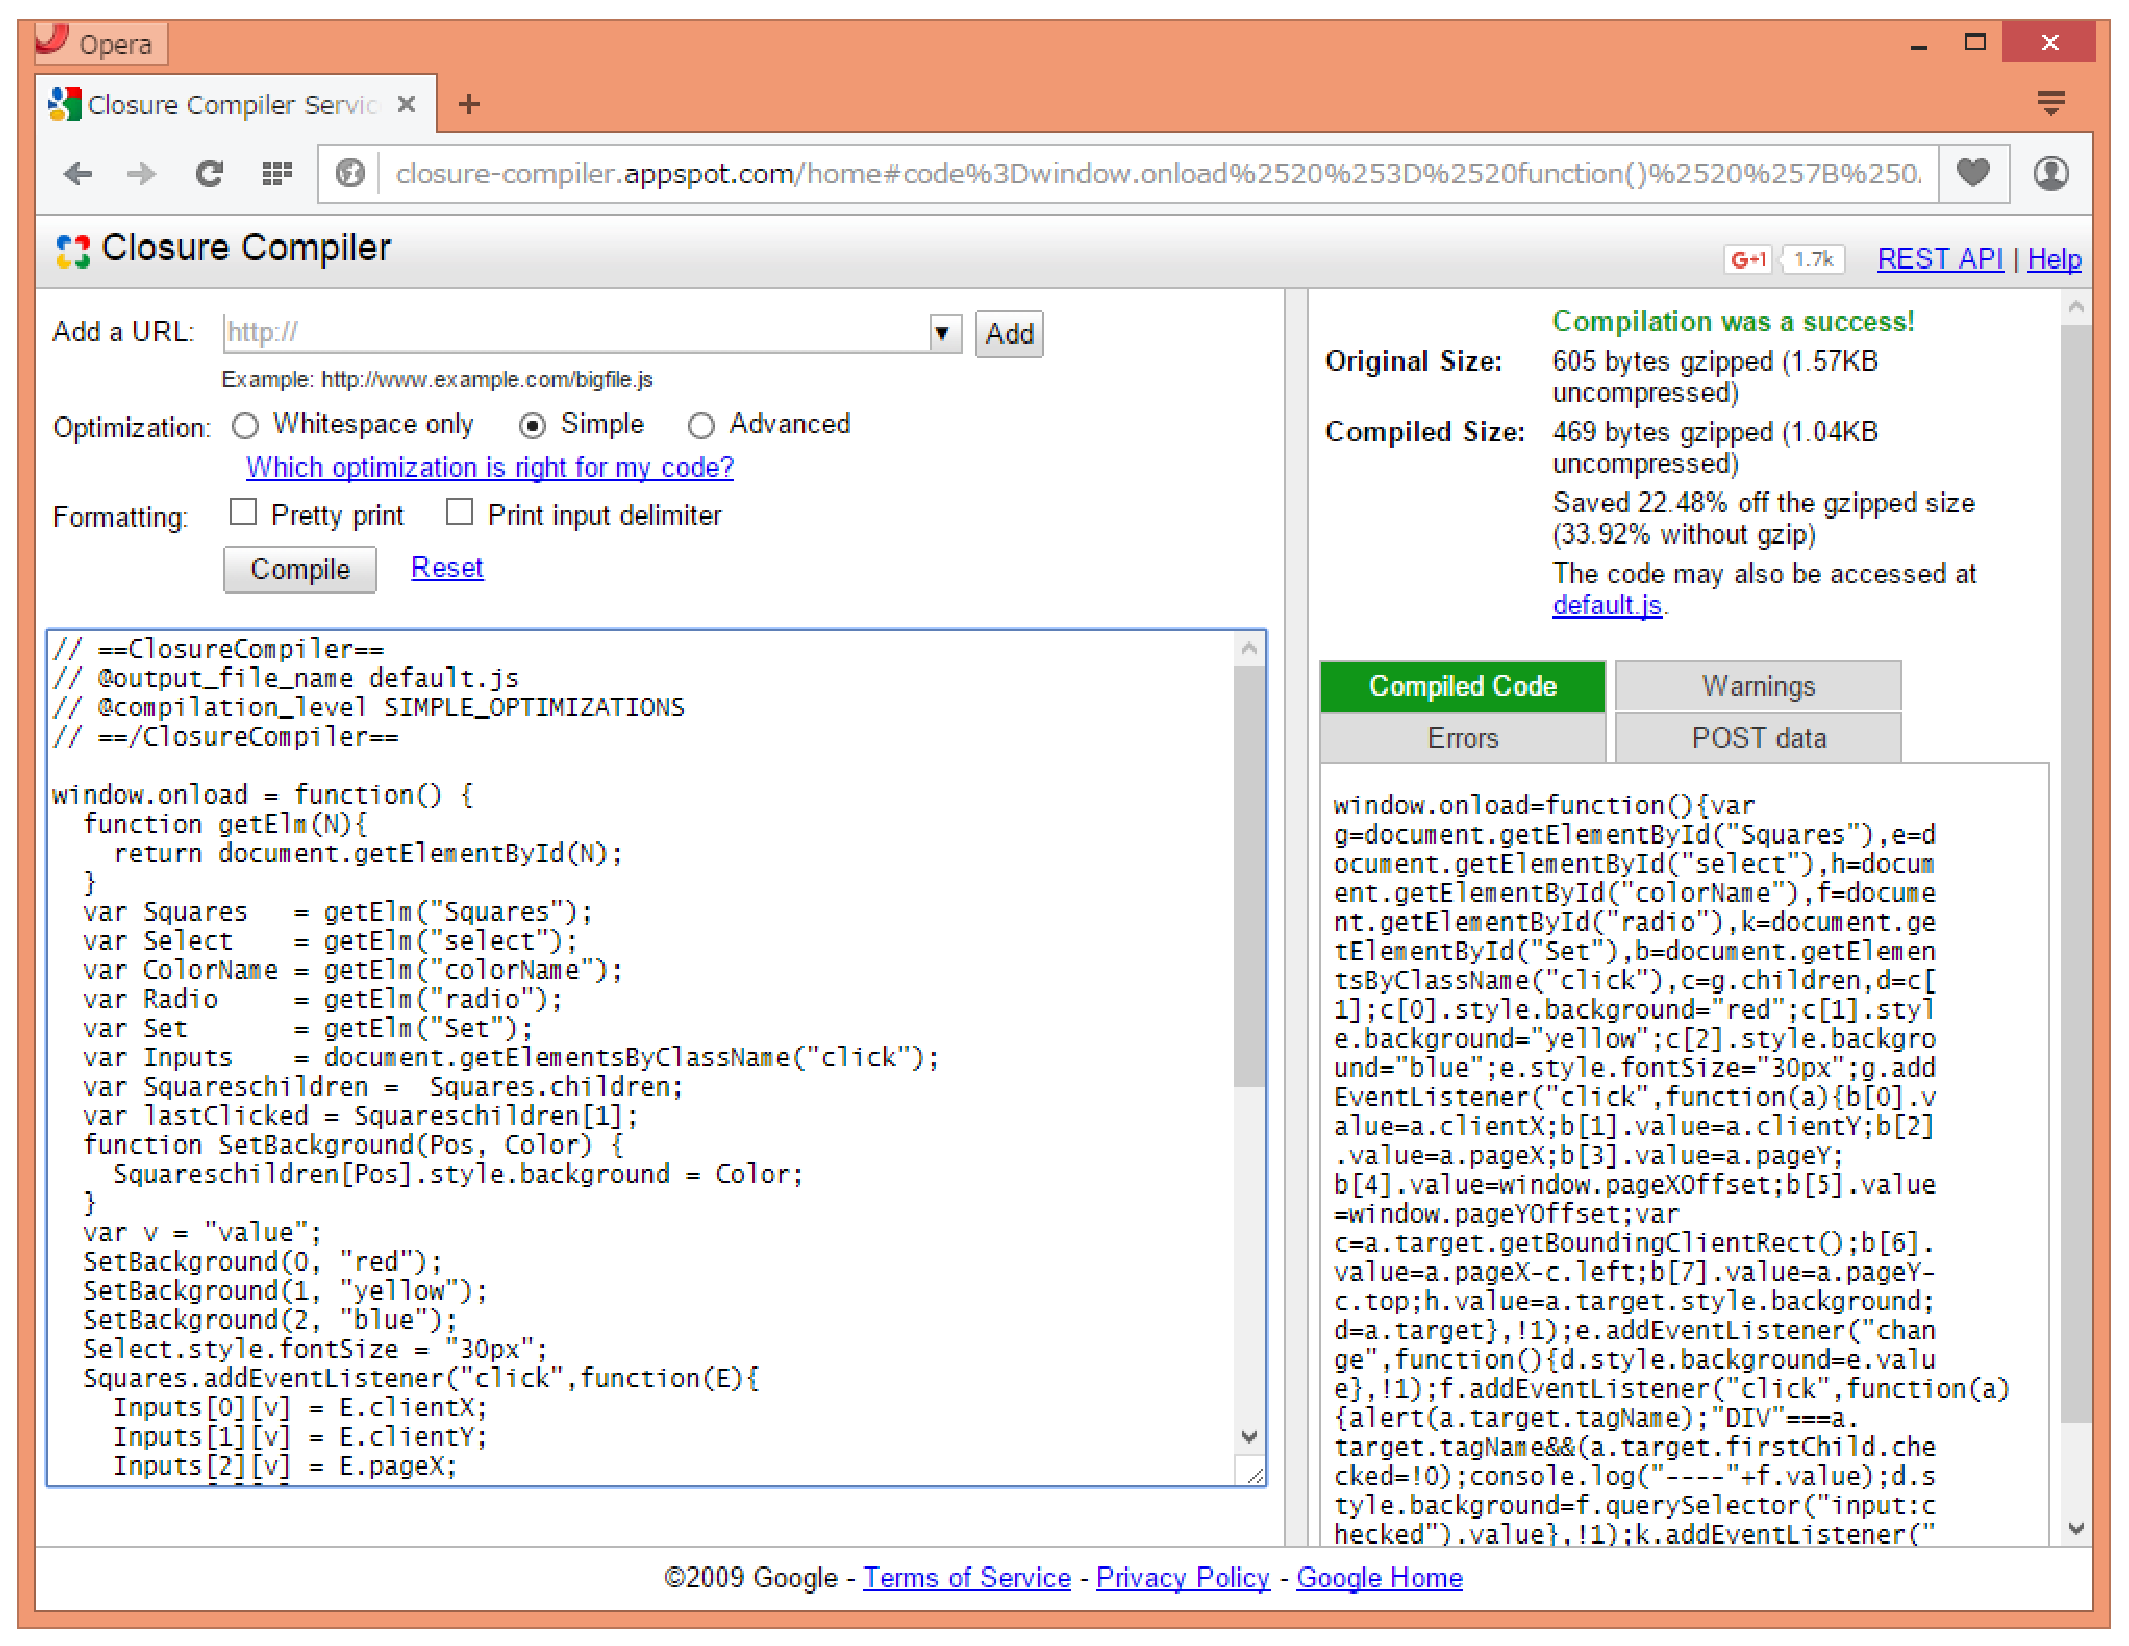
\includegraphics[width=1\textwidth]{10-01closur-compiler-res02.eps}
	\end{center}
 \caption{Closure Compiler の結果}\label{closure-compiler-res02}
 \end{figure}

 画面の右のほうで、元のファイルの大きさが1.53KBであったのに対し、短縮化
 の結果が1.06KBとなったことがわかる。

 短縮化の効果を見るために、対応するコードのところに改行を入れたものが次
 のリストである。
 \begin{Verbatim}[numbers=left]
window.onload=function(){var b=document.getElementById("Squares"),
  e=document.getElementById("select"),
  g=document.getElementById("colorName"),
  f=document.getElementById("radio"),
  h=document.getElementById("Set"),
  c=document.getElementsByClassName("click"),
  d=b.children[1];
  b.children[0].style.background="red";
  b.children[1].style.background="yellow";
  b.children[2].style.background="blue";
  e.style.fontSize="30px";
  b.addEventListener("click",function(a){
    c[0].value=a.clientX;
    c[1].value=a.clientY;
    c[2].value=a.pageX;
    c[3].value=a.pageY;
    c[4].value=window.pageXOffset;
    c[5].value=window.pageYOffset;
    var b=a.target.getBoundingClientRect();
    c[6].value=a.pageX-b.left;
    c[7].value=a.pageY-b.top;
    g.value=a.target.style.background;d=a.target},!1);
    e.addEventListener("change",function(){d.style.background=e.value},!1);
    f.addEventListener("click",function(a){
      alert(a.target.tagName);
      "DIV"===a.target.tagName&&(a.target.firstChild.checked=!0);
      console.log("----"+f.value);
      d.style.background=f.querySelector("input:checked").value},!1);
    h.addEventListener("click",function(){d.style.background=g.value},!1)};
\end{Verbatim}

ここで行われている短縮化は次のとおりである。
\begin{itemize}
 \item 空白の除去
 \item 変数宣言をまとめる。
 \item 変数名の単純化
 \item いくつかの定数を短いものに変える。

			 \texttt{false}は\texttt{!1}に変えている(5文字から2文字)。
 \item \texttt{if}文の簡略化

短縮化後の29行目は\texttt{if}文であったものが論理式の\verb+&&+で置き換え
			 られている。
\end{itemize}
この一方で\texttt{document.getElementById}などはシステムで定義されている
のでそのまま短縮化、共通化できない。この部分も短くするためにはソースコー
ドに工夫が必要である。

しかし、\texttt{document.getElementById}をラップする関数を定義してプログラムコー
 ドを短くしてもうまくいかない。
 \begin{Verbatim}
  function getElm(N){
    return document.getElementById(N);
  }
  var Squares   = getElm("Squares");
  var Select    = getElm("select");
	...
 \end{Verbatim}
 図\ref{closure-compiler-res03}がコンパイルの結果である。
 \begin{figure}[ht]
	\begin{center}
	 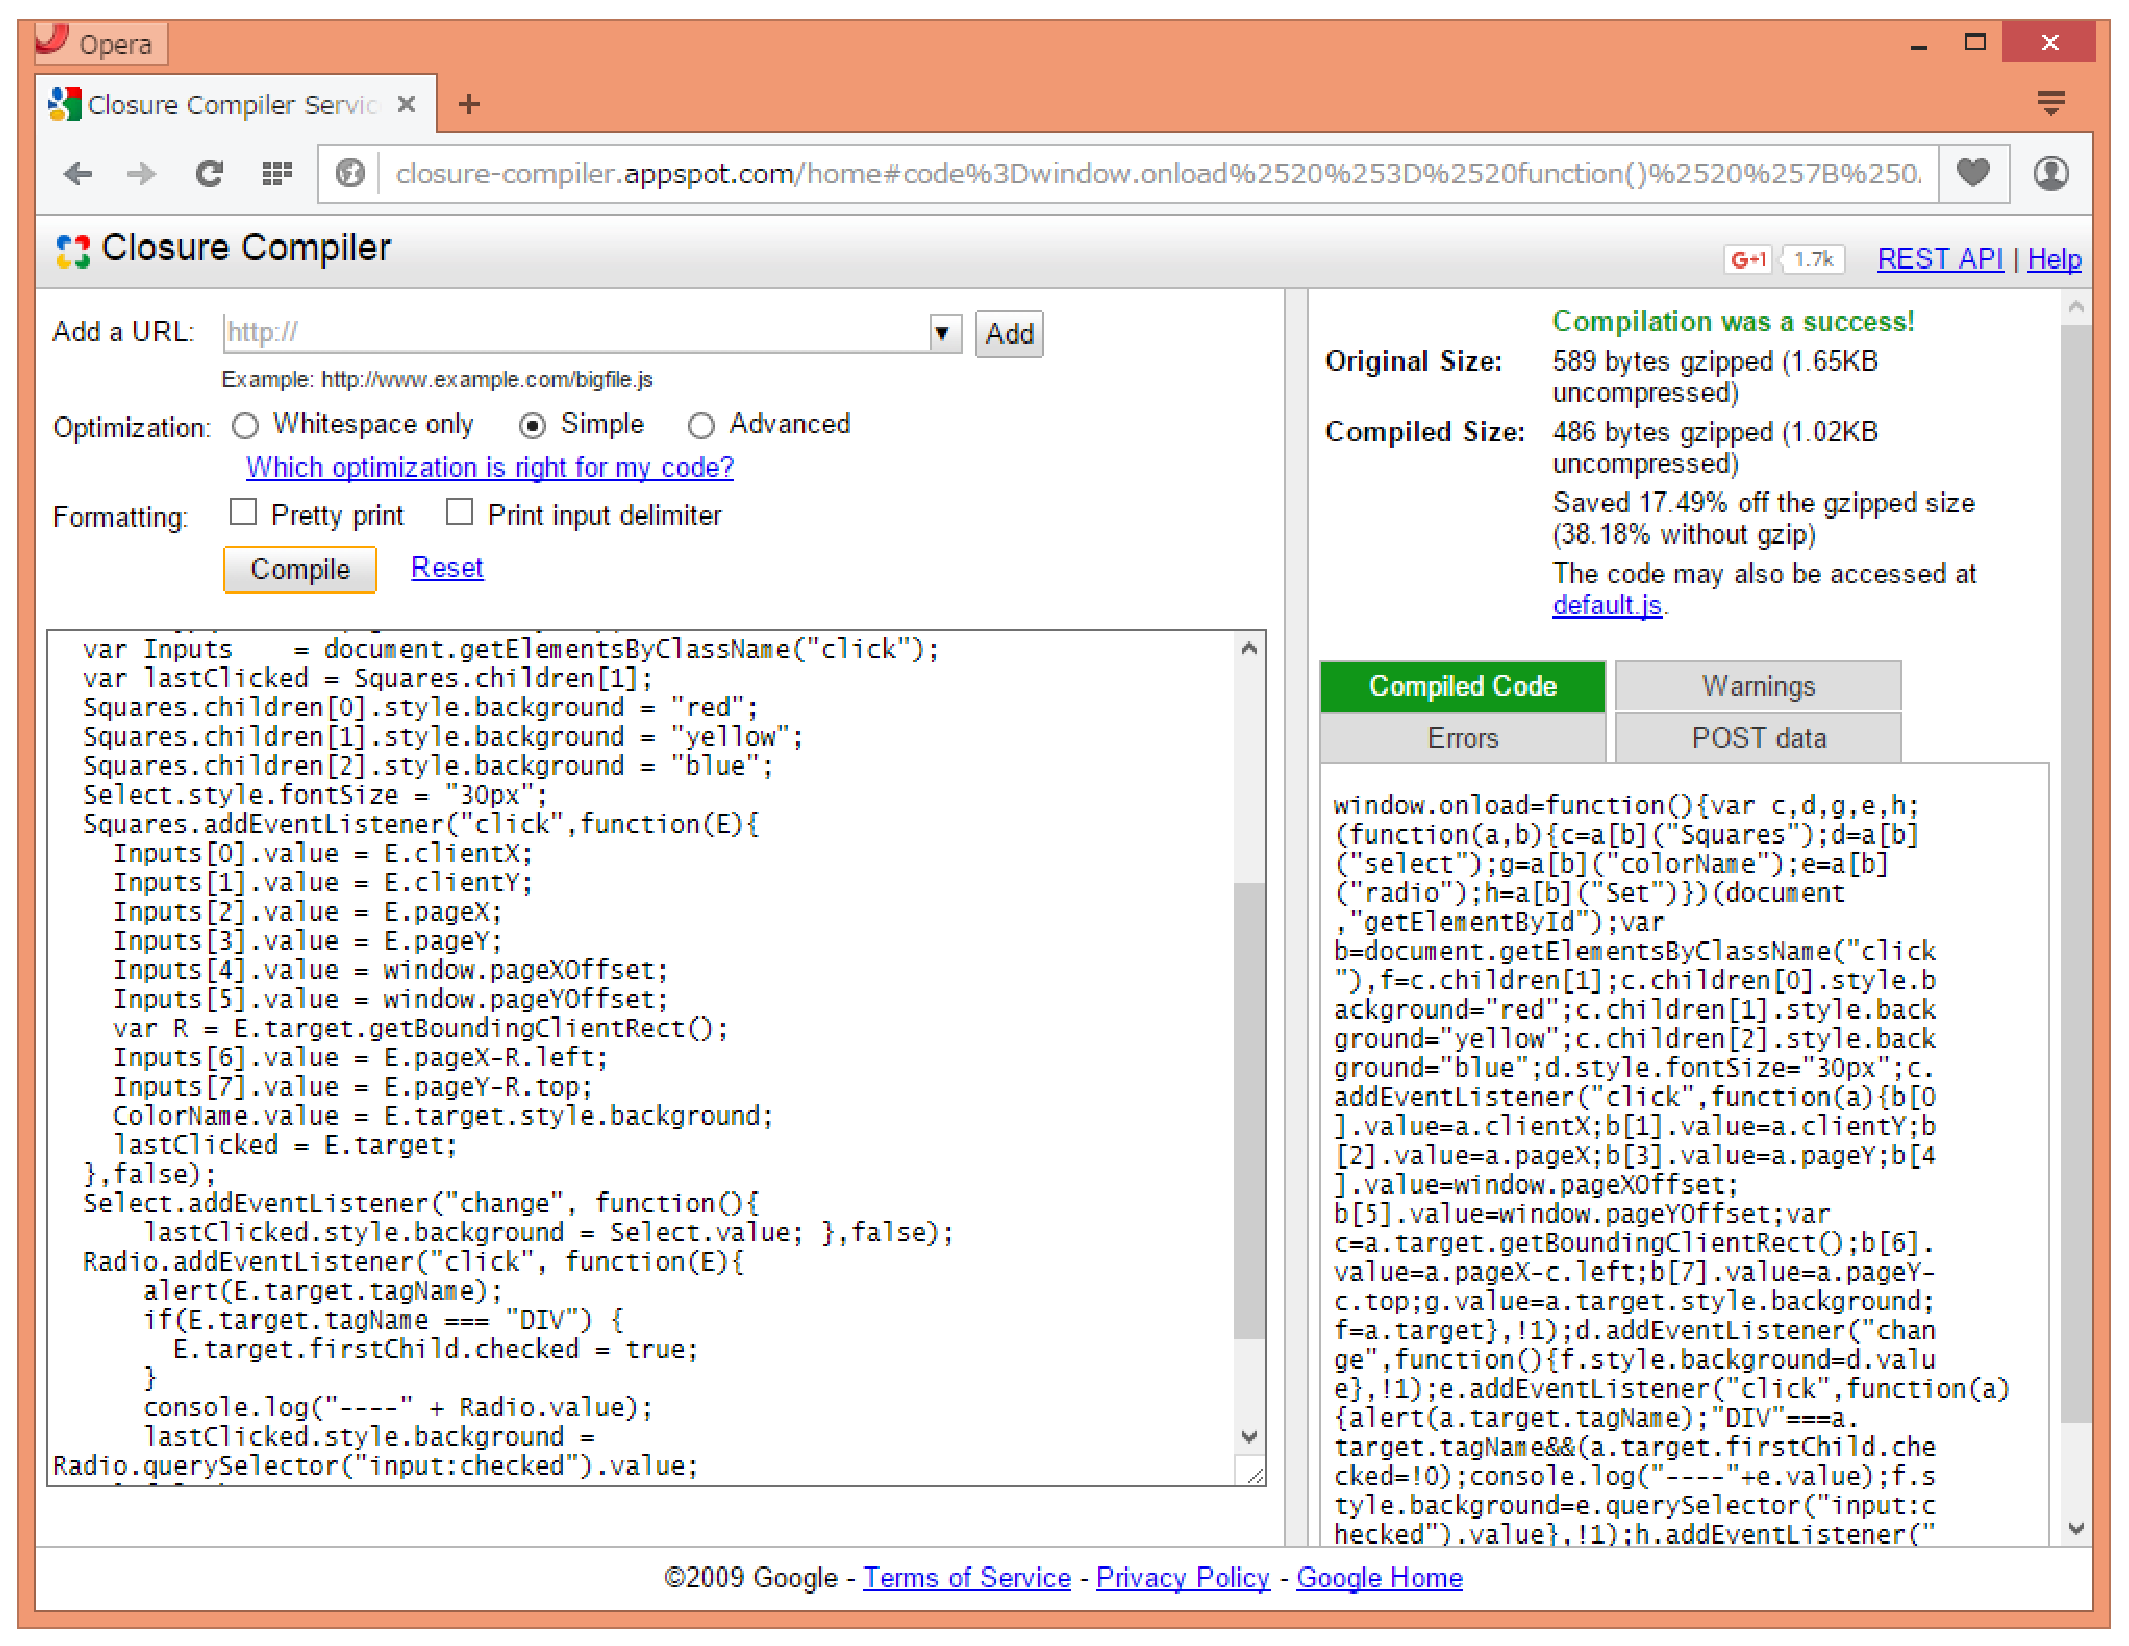
\includegraphics[width=1\textwidth]{10-01closur-compiler-res03.eps}
	\end{center}
 \caption{Closure Compiler の結果(2)}\label{closure-compiler-res03}
 \end{figure}

 コンパイルの結果を見ると、ラップした関数は消えていて、もとの
 \texttt{document.getElementById}に戻っている。
 
 これを避けるためには関数の引数に
 \texttt{document}と\texttt{document.getElementById}を渡すことで解決できる。
このとき、引数で渡された\texttt{document.getElementById}の実行時の\texttt{this}が
 \texttt{document}にならないので、\texttt{call}を用いて\texttt{this}を
 \texttt{document}にする必要がある。また、関数は1度実行する必要がある。

 次のリストはそのように書き直したものである。
\begin{Verbatim}
  var Squares, Select, ColorName, Radio, Set;
  (function(document,getElementById){
      Squares   = getElementById.call(document,"Squares");
      Select    = getElementById.call(document,"select");
      ColorName = getElementById.call(document,"colorName");
      Radio     = getElementById.call(document,"radio");
      Set       = getElementById.call(document,"Set");
	})(document,document.getElementById);
\end{Verbatim}
図\ref{closure-compiler-res04}がその結果である。
 \begin{figure}[ht]
	\begin{center}
	 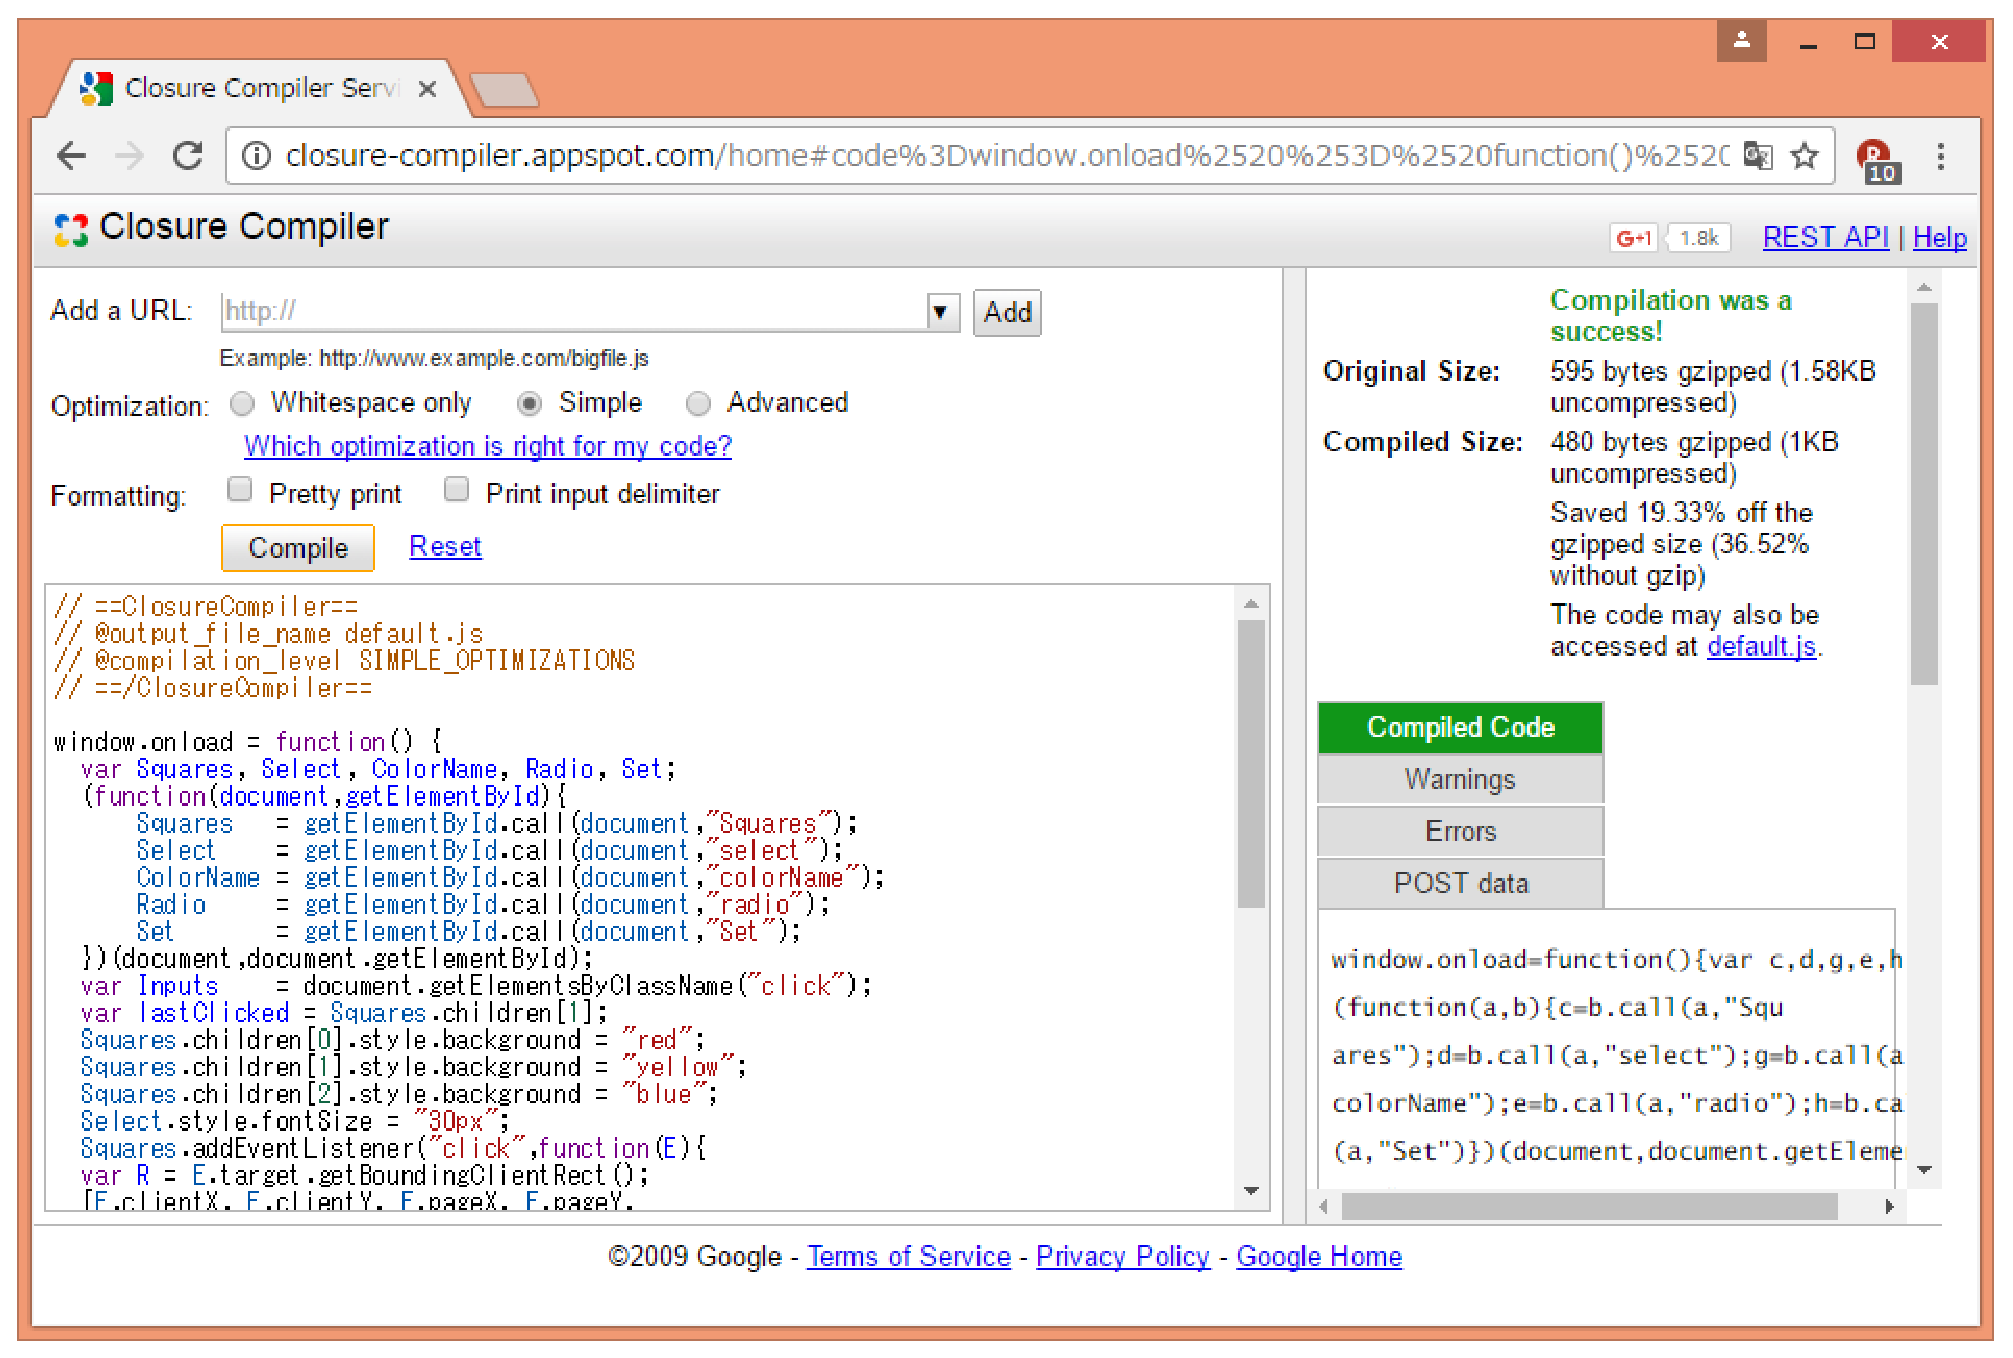
\includegraphics[width=1\textwidth]{10-01closur-compiler-res04.eps}
	\end{center}
 \caption{Closure Compiler の結果(3)}\label{closure-compiler-res04}
 \end{figure}
 コンパイル後の結果が1KBとわずかに小さくなっていることがわかる。

 この部分の短縮化のコードは次のようになっている。
\begin{Verbatim}
var c,d,g,e,h;
  (function(a,b){c=b.call(a,"Squares");d=b.call(a,"select");
  g=b.call(a,"colorName");e=b.call(a,"radio");
  h=b.call(a,"Set")})(document,document.getElementById)
\end{Verbatim}
このようにシステムで定義されたメソッドやプロパティを関数の引数として渡す
と短縮化の効率が上がる。また、これによりソースコードの理解が難しくなる。

\section{Webサイトの効率化}
\subsection{Contents Deliverly Network(CDN)}
jQueryの短縮化はファイルサイズを減らすことでWebサイトの負荷も減らしてい
る。さらに、このようなファイルはいろいろなサイトで使用されているのでクラ
イアント側でもキャッシュしておけばダウンロードの回数を減らせば、回線の負
荷が減る。このためには、ライブラリーを置いておくサイトを用意し、そこのファ
イルを参照すればよい。このような目的のサイトをContents Deliverly
Network(CDN)と呼ぶ。jQueryの場合は
\texttt{https://code.jquery.com/jquery-3.1.1.min.js}が短縮化されたファイ
ルのCDNの一つである。
\subsection{CSS Sprite}
Yahoo Japan のトップページには小さな画像がたくさんある。ブラウザは表示し
ようとするページに画像があれば、そのページのサイトに画像を要求しに行く。
したがって、表示する画像が多いとその回数分だけ、サーバーと通信が行われる。
このことはサーバーに負荷がかかる。これを避けるためにブラウザは最近ダウン
ロードしたファイルを保存して、同じものが要求されたときには、サーバーに要
求しないで、保存してあるファイルを使用する(キャッシュの利用)。

この機能を
利用してサーバーは、小さな画像が複数含まれる単一の大きな画像を用意し、そ
の一部だけをページに表示するページを用意する。この方法で画像を表示するた
めにはCSSのbackground機能を利用する。これをCSS Sprite と呼ぶ。

Yahoo Japan のソースコードで \texttt{background-image} をキーワードに検
索すればCSS Sprite で使用されている画像が見つかるであろう。

なお、Yahoo Japan などのアクセスが多いサイトではサーバーとの通信の回数を
減らす目的でCSSファイルやJavaScriptのファイルは外部ファイルにしていない
ので合わせて確認してほしい。